\documentclass[nototal]{beamer}
%\documentclass[nototal,handout]{beamer}

% This file is a solution template for:

% - Talk at a conference/colloquium.
% - Talk length is about 20min.
% - Style is ornate.


%
% In principle, this file can be redistributed and/or modified under
% the terms of the GNU Public License, version 2.
%
% However, this file is supposed to be a template to be modified
% for your own needs. For this reason, if you use this file as a
% template and not specifically distribute it as part of a another
% package/program, I grant the extra permission to freely copy and
% modify this file as you see fit and even to delete this copyright
% notice. 


\mode<presentation>
{
  %\usetheme{Madrid}
 \usetheme{Boadilla}
  % or ...

  \setbeamercovered{transparent}
  % or whatever (possibly just delete it)
}

\usepackage{verbatim}
\usepackage[english]{babel}
% or whatever

\usepackage[latin1]{inputenc}
% or whatever

%\usepackage{bar}
\usepackage{times}
\usepackage[T1]{fontenc}
% Or whatever. Note that the encoding and the font should match. If T1
% does not look nice, try deleting the line with the fontenc.
\usepackage{graphicx} %sjr added
\graphicspath{{figures/}}
\usepackage{hyperref}

\author{\textsc{Sergio Rey}}
\institute[ASU]{\textbf{GPH 483/598}\\\textbf{Geographic Information
Analysis}\\School of Geographical Sciences and Urban Planning\\Arizona State
University\\Spring 2010}
\title[Spatial Dependence]{Spatial Dependence}
\subtitle{}
\date[GPH 483]{}


% - Either use conference name or its abbreviation.
% - Not really informative to the audience, more for people (including
%   yourself) who are reading the slides online

% This is only inserted into the PDF information catalog. Can be left
% out. 



% If you have a file called "university-logo-filename.xxx", where xxx
% is a graphic format that can be processed by latex or pdflatex,
% resp., then you can add a logo as follows:

% \pgfdeclareimage[height=0.5cm]{university-logo}{university-logo-filename}
% \logo{\pgfuseimage{university-logo}}



% Delete this, if you do not want the table of contents to pop up at
% the beginning of each subsection:
\AtBeginSubsection[]
{
  \begin{frame}<beamer>
    \frametitle{Outline}
    \tableofcontents[currentsection,currentsubsection]
  \end{frame}
}


% If you wish to uncover everything in a step-wise fashion, uncomment
% the following command: 

%\beamerdefaultoverlayspecification{<+->}


\begin{document}

\begin{frame}
  \titlepage
\end{frame}

\begin{frame}
  \frametitle{Outline}
  \tableofcontents
  % You might wish to add the option [pausesections]
\end{frame}


% Structuring a talk is a difficult task and the following structure
% may not be suitable. Here are some rules that apply for this
% solution: 

% - Exactly two or three sections (other than the summary).
% - At *most* three subsections per section.
% - Talk about 30s to 2min per frame. So there should be between about
%   15 and 30 frames, all told.

% - A conference audience is likely to know very little of what you
%   are going to talk about. So *simplify*!
% - In a 20min talk, getting the main ideas across is hard
%   enough. Leave out details, even if it means being less precise than
%   you think necessary.
% - If you omit details that are vital to the proof/implementation,
%   just say so once. Everybody will be happy with that.
\section{Concepts and Issues}
\begin{frame}[<+->]
  \frametitle{Spatial Dependence }
  \begin{quote}
There is no question with respect to emergent geospatial science. The important harbingers were Geary's article on spatial autocorrelation, Dacey's paper about two- and K-color maps, and that of Bachi on geographic series.

-- Berry, Griifth, Tiefelsdorf (2008)

  \end{quote}
 \end{frame}

\begin{frame}[<+->]
  \frametitle{Spatial Dependence}
  \begin{block}{Working Concept}
    \begin{itemize}
      \item what happens at one place depends on events in nearby places
      \item all things are related but nearby things are more related than
        distant things (Tobler)
    \end{itemize}
   \end{block}
\begin{block}{Goodchild 1991}
    \begin{itemize}
      \item a world without positive spatial dependence would be an impossible
        world
      \item impossible to describe
      \item impossible to live in
      \item \alert{hell} is a place with \alert{no} spatial dependence
    \end{itemize}
   \end{block}
 \end{frame}

 \begin{frame}
   \frametitle{Spatial Dependence}
\begin{block}{Categorizing}
    \begin{itemize}
      \item Type: Substantive versus nuisance
      \item Direction: Positive versus negative
    \end{itemize}
  \end{block}

\begin{block}{Issues}
    \begin{itemize}
      \item Time versus space
      \item Inference
    \end{itemize}
  \end{block}
 \end{frame}

 \begin{frame}[<+->]
   \frametitle{Substantive Spatial Dependence}
   \begin{block}{Process Based}
     \begin{itemize}
       \item Part of the process under study
       \item Leaving it out
         \begin{itemize}
           \item Incomplete understanding
           \item Biased inferences
         \end{itemize}
     \end{itemize}
    \end{block}
  \end{frame}


 \begin{frame}[<+->]
   \frametitle{Nuisance Spatial Dependence}
   \begin{block}{Not Process Based}
     \begin{itemize}
       \item Artifact of data collection
       \item Process boundaries not matching data boundaries
       \item Scattering across pixels
       \item GIS induced
     \end{itemize}
    \end{block}
  \end{frame}


  \begin{frame}
    \frametitle{Boundary}
    \begin{center}
      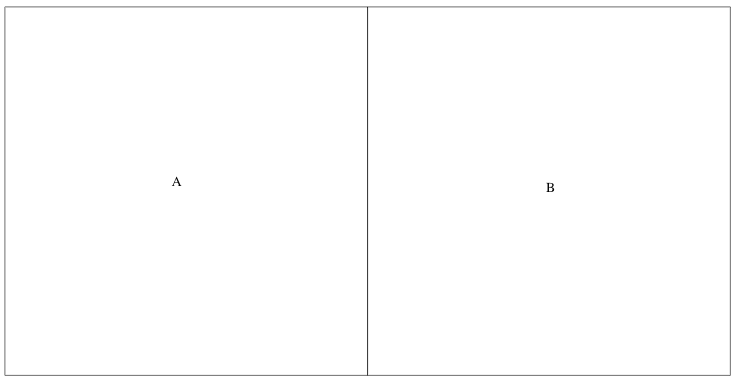
\includegraphics[width=.65\linewidth]{boundary.png}
    \end{center}
  \end{frame}


  \begin{frame}
    \frametitle{Boundary Mismatch}
    \begin{center}
      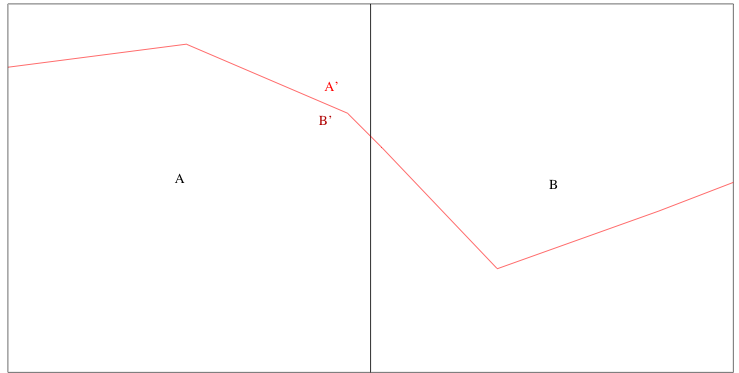
\includegraphics[width=.65\linewidth]{boundary2.png}
    \end{center}

    \begin{itemize}
      \item Even if $A$ and $B$ are independent
      \item $A'$ and $B'$ will be dependent
    \end{itemize}
  \end{frame}

\begin{frame}
    \frametitle{Nusiance vs. Substantive Dependence}
    \begin{block}{Issues}
    \begin{itemize}
      \item Not always easy to differentiate from substantive
      \item Different implications for each type
      \item Specification strategies (Econometrics)
      \item Both can be operating jointly
    \end{itemize}
  \end{block}
  \end{frame}


\begin{frame}
    \frametitle{Space versus Time}
    \begin{block}{Temporal Dependence}
    \begin{itemize}
      \item Past influences the future
      \item Recursive
      \item One dimension
    \end{itemize}
  \end{block}
\begin{center}
      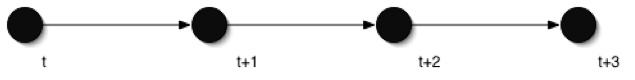
\includegraphics[width=.65\linewidth]{timerecursive.png}
    \end{center}

  \end{frame}

\begin{frame}
    \frametitle{Space versus Time}
    \begin{block}{Spatial Dependence}
    \begin{itemize}
      \item Multi-directional
      \item Simultaneous
    \end{itemize}
  \end{block}
\begin{center}
      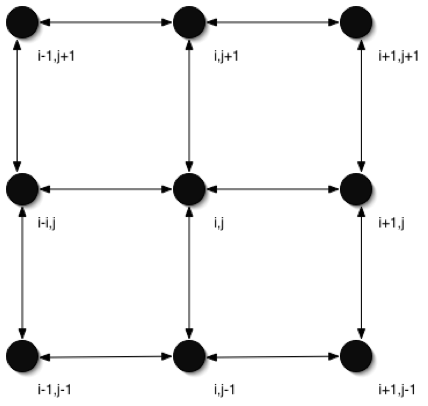
\includegraphics[width=.55\linewidth]{spacesimultaneous.png}
    \end{center}


  \end{frame}


\begin{frame}
    \frametitle{Terminology}
    \begin{block}{Related Concepts}
    \begin{itemize}
      \item Spatial Dependence
      \item Spatial Autocorrelation
      \item Spatial Association
    \end{itemize}
  \end{block}
  \end{frame}

\begin{frame}
    \frametitle{Spatial Dependence}
    \begin{block}{Distributional Characteristic}
    \begin{itemize}
      \item Multivariate density function
      \item difficult/impossible to verify empirically
    \end{itemize}
  \end{block}
    \begin{block}{Dependent Distribution}
      \begin{itemize}
        \item does not factor in marginal densities
      \end{itemize}
    \end{block}
  \end{frame}


\begin{frame}
    \frametitle{Spatial Autocorrelation}
    \begin{itemize}
      \item Auto = same variable
      \item Correlation = scaled covariance
      \item Spatial - geographic pattern to the correlation
    \end{itemize}
  \end{frame}


\begin{frame}
    \frametitle{Spatial Autocorrelation}
    \begin{block}{Measurement of Moment of Distribution}
    \begin{itemize}
      \item off-diagonal elements of variance-covariance matrix
      \item autocovariance
      \item $C[y_i,y_j] \ne 0 \ \forall i\ne j$
      \item can be estimated
    \end{itemize}
  \end{block}
  \begin{block}{Spatial Autocorrelation Coefficient}
    \begin{itemize}
      \item significance test on coefficient = 0
    \end{itemize}
  \end{block}
  \end{frame}

\begin{frame}
    \frametitle{Spatial Autocorrelation}
    \begin{block}{Joint multivariate distribution function}
      \begin{equation}
f(y) = \frac{ \exp\left[
-\frac{1}{2}
(y-\mu)'
\Sigma^{-1}
(y-\mu)
\right]} 
{\sqrt{(2\pi)^n|\Sigma|}}
      \end{equation}
  \end{block}
    \end{frame}


\begin{frame}
    \frametitle{Variance-Covariance Matrix}
    \begin{equation}
\Sigma=
\left[
\begin{array}{rrrr}
\sigma_{1,1}&\sigma_{1,2}&\ldots&\sigma_{1,n}\\
\sigma_{2,1}&\sigma_{2,2}&\ldots&\sigma_{2,n}\\
\vdots&\vdots&\ddots&\vdots\\
\sigma_{n,1}&\sigma_{n,2}&\ldots&\sigma_{n,n}
\end{array}
\right]
    \end{equation}
    \begin{itemize}
      \item covariance: $\sigma_{i,j} = E[(y_i - \mu_i)(y_j-\mu_j)      ]$
      \item symmetry:  $\sigma_{i,j} =\sigma_{i,j}$
      \item variance: $\sigma_{i,i} = E[(y_i - \mu_i)(y_i-\mu_i)      ]$
    \end{itemize}
    \end{frame}


\begin{frame}
    \frametitle{Correlation}
    \begin{equation}
      \rho_{ij} = \frac{\sigma_{ij}}{\sqrt{\sigma_{i}^2}\sqrt{\sigma_{j}^2}}
    \end{equation}
    \begin{equation}
    -1.0 \le \rho_{ij} \le 1.0
    \end{equation}
    \end{frame}


\begin{frame}
    \frametitle{Data Types and Autocorrelation}
    \begin{block}{Point Data}
      \begin{itemize}
        \item focus on geometric pattern
        \item random vs. nonrandom
        \item clustered vs. uniform
      \end{itemize}
    \end{block}
    \begin{block}{Geostatistics}
      \begin{itemize}
        \item 2-D modeling of spatial covariance (pairs of observations in
          function of distance)
        \item kriging, spatial prediction
      \end{itemize}
    \end{block}
\end{frame}


\begin{frame}
    \frametitle{Data Types and Autocorrelation}
    \begin{block}{Lattice Data}
      \begin{itemize}
        \item areal units: states, counties, census tracts, watersheds
        \item points: centroids of areal units
        \item focus on the spatial nonrandomness of attribute values
      \end{itemize}
    \end{block}
\end{frame}


\begin{frame}
    \frametitle{Spatial Association}
    \begin{block}{Not a Rigorously Defined Term}
      \begin{itemize}
        \item Usually the same as spatial autocorrelation
        \item often used in non-technical discussion
        \item avoid unless meaning is clear
      \end{itemize}
    \end{block}
\end{frame}

\begin{frame}
    \frametitle{Spatial Dependence}
    \begin{block}{Good News (for geographers)}
      \begin{itemize}
        \item Space matters
        \item Suggestive of underlying process
      \end{itemize}
    \end{block}
    \begin{block}{Bad news}
      \begin{itemize}
        \item invalidates random sampling assumption
        \item necessitates new methods = spatial statistics and spatial
          econometrics
      \end{itemize}

    \end{block}
\end{frame}

\begin{frame}
    \frametitle{Spatial Dependence: Implications}

The specific process we are simulating is as follows:\begin{eqnarray}\label{eq:simdgp}y&=&X\beta + \epsilon \\ \nonumber\epsilon &=& \lambda W \epsilon + \nu  \end{eqnarray}
where $\nu^{\sim}N(0,\sigma^{2}I)$, $\lambda$ is a spatial autocorrelation parameter (scalar) and $W$
is a spatial weights matrix. We will shortly explain these new entities,
but for now we simply note that they allow us to simulate a process
whereby the $\epsilon$'s, and therefore the $y$'s are spatially
autocorrelated. If $\lambda=0$ then the $i.i.d.$ assumption holds,
otherwise there is spatial dependence.

$\beta=40, \ \sigma^2=16, \ x=[1,1,\ldots]$

$\lambda=[0.0, 0.25, 0.50, 0.75], \ n=25$
\end{frame}

\begin{frame}
    \frametitle{Spatial Dependence: Implications}


For each D.G.P. we are going to generate 500 samples of size $n=25$ for
our map. You can think of this as generating 500 maps using the same
D.G.P.. For each sample we will then do the following:
\begin{enumerate}
        \item Estimate $\mu$ with $\bar{y}$
        \item Test the hypothesis that $\mu=40$
\end{enumerate}

\end{frame}

\begin{frame}
  \frametitle{Implications}
\begin{table}\caption{Monte Carlo Results}\label{t:sasim}
\begin{center}
\begin{tabular}{  rrrrr  }
\hline
$\lambda$ & 0.00 & 0.25 & 0.50 & 0.75 \\ 
\hline
$\hat{\mu}$ & 39.947 & 39.931 & 39.901 & 39.814 \\
$\sigma_{\bar{x}}$ & 0.816 & 1.090 & 1.641& 3.304 \\
$p$ & 0.056 & 0.148 & 0.278 & 0.492 \\
\hline  
\end{tabular}
\end{center}
\end{table}
\end{frame}

\section{Null and Alternative Hypotheses}

\begin{frame}
  \frametitle{Spatial Randomness}
  \begin{block}{Null Hypothesis}
    \begin{itemize}
      \item observed spatial pattern of values is equally likely as any other
        spatial pattern
      \item values at one location do no depend on values at other
        (neighboring) locations
      \item under spatial randomness, the location of values may be altered
        without affecting the information content of the data
    \end{itemize}
  \end{block}
\end{frame}

  \begin{frame}
    \frametitle{Spatial Autocorrelation on a Grid}
    \begin{center}
      \begin{figure}
      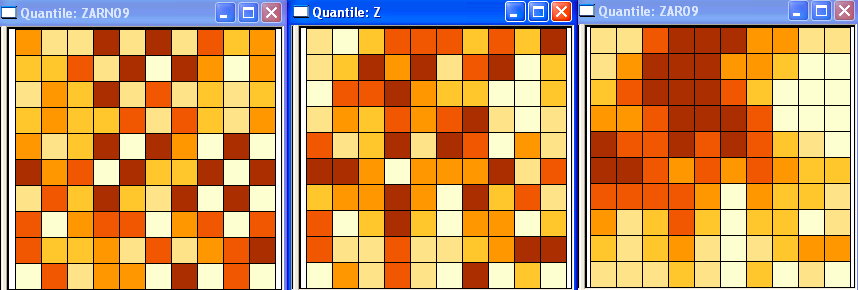
\includegraphics[width=.65\linewidth]{patterns.png}
      \caption{Negative, Random, Positive}
    \end{figure}
    \end{center}
  \end{frame}


\begin{frame}
  \frametitle{Positive Spatial Autocorrelation}
  \begin{block}{Clustering}
    \begin{itemize}
      \item like values tend to be in similar locations
    \end{itemize}
  \end{block}
  \begin{block}{Neighbor similarity}
    \begin{itemize}
      \item more alike than they would be under spatial randomness
    \end{itemize}
  \end{block}
\begin{block}{Compatible with Diffusion}
    \begin{itemize}
      \item but not necessarily caused by diffusion
    \end{itemize}
  \end{block}
\end{frame}


  \begin{frame}
    \frametitle{Positive Spatial Autocorrelation}
    \begin{center}
      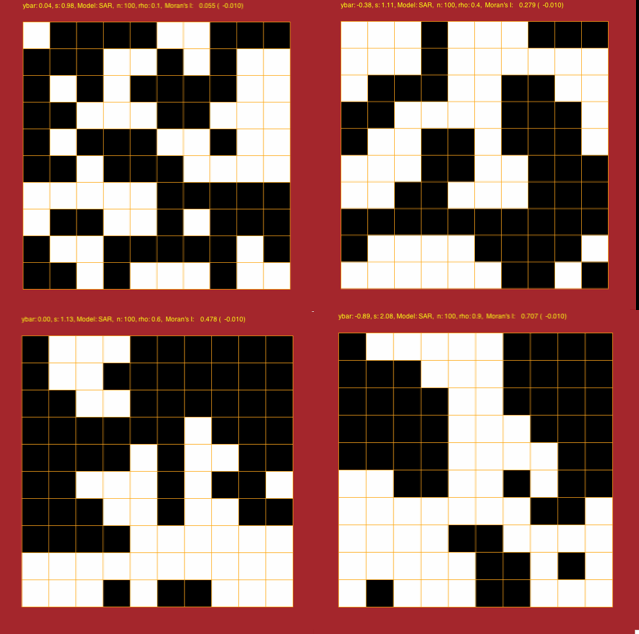
\includegraphics[width=.65\linewidth]{positive.png}
    \end{center}
  \end{frame}

\begin{frame}
  \frametitle{Negative Spatial Autocorrelation}
  \begin{block}{Checkerboard pattern}
    \begin{itemize}
      \item anti-clustering
    \end{itemize}
  \end{block}
  \begin{block}{Neighbor dissimilarity}
    \begin{itemize}
      \item more dissimilar than they would be under spatial randomness
    \end{itemize}
  \end{block}
\begin{block}{Compatible with Competition}
    \begin{itemize}
      \item but not necessarily caused by competition
    \end{itemize}
  \end{block}
\end{frame}

  \begin{frame}
    \frametitle{Negative Spatial Autocorrelation}
    \begin{center}
      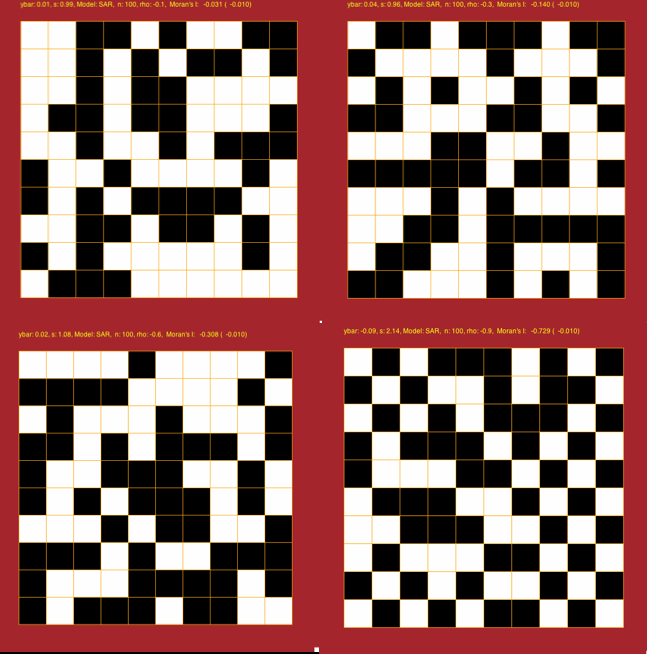
\includegraphics[width=.65\linewidth]{negative.png}
    \end{center}
  \end{frame}

\begin{frame}
  \frametitle{Autocorrelation and Diffusion}
  \begin{block}{One does not necessarily imply the other}
    \begin{itemize}
      \item diffusion tends to yield positive spatial autocorrelation but the
	reverse is not necessary
      \item positive spatial correlation may be due to structural factors,
	without contagion or diffusion
    \end{itemize}
  \end{block}
\end{frame}

\begin{frame}
  \frametitle{True vs. Apparent Contagion}
  \begin{block}{What is the Cause behind the clustering?}  
    \begin{itemize}
      \item True contagion
	\begin{itemize}
	  \item result of a contagious process, social interaction, dynamic
	    process
	\end{itemize}
      \item Apparent contagion
	\begin{itemize}
	  \item spatial heterogeneity
	  \item stratification
	\end{itemize}
      \item Cannot be distinguished in a pure cross section
      \item Equifinality or Identification Problem
    \end{itemize}
  \end{block}
\end{frame}

\section{Spatial Autocorrelation Tests}

\begin{frame}
  \frametitle{Clustering}
  \begin{block}{Global characeristic}
    \begin{itemize}
      \item property of overall pattern = all observations
      \item are like values more grouped in space than random
      \item test by means of a global spatial autocorrelation statistic
      \item no location of the clusters determined
    \end{itemize}
   \end{block}
 \end{frame}


\begin{frame}
  \frametitle{Clusters}
  \begin{block}{Local characeristic}
    \begin{itemize}
      \item where are the like values more grouped in space than random?
      \item property of local pattern = location-specific
      \item test by means of a local spatial autocorrelation statistic
      \item local clusters may be compatible with global spatial randomness
    \end{itemize}
   \end{block}
 \end{frame}

\begin{frame}
  \frametitle{Spatial Autocorrelation Statistic}
  \begin{block}{Structure}
    \begin{itemize}
      \item Formal Test of Match between Value Similarity and Locational
	Similarity
      \item Statistic Summarizes Both Aspects
      \item Significance
	\begin{itemize}
	  \item how likely is it (p-value) that the computed statistic would
	    take this (extreme) value in a spatially random pattern
	\end{itemize}
    \end{itemize}
   \end{block}
 \end{frame}

\begin{frame}
  \frametitle{Attribute Similarity}
    \begin{itemize}
      \item Summary of the similarity or dissimilarity of a variable at
	different locations
	\begin{itemize}
	  \item variable $y$ at locations $i,j$ with $i\ne j$
	\end{itemize}
      \item Measures of similarity
	\begin{itemize}
	  \item cross product: $y_i y_j$
	\end{itemize}
      \item Measures of dissimilarity
	\begin{itemize}
	  \item squared differences: $(y_i - y_j)^2$
	  \item absolute differences: $|y_i - y_j|$
	\end{itemize}
    \end{itemize}
 \end{frame}

\begin{frame}
  \frametitle{Locational Similarity}
    \begin{itemize}
      \item Formalizing the notion of Neighbor
	\begin{itemize}
	  \item when two spatial units a-priori are likely to interact
	\end{itemize}
      \item Spatial Weights
	\begin{itemize}
	  \item not necessarility geographical
	  \item many approaches
	\end{itemize}
    \end{itemize}
 \end{frame}

 \begin{frame}
   \frametitle{Summary}
   \begin{block}{Spatial Dependence}
     \begin{itemize}
       \item Core of Lattice Analysis
       \item Spatial Autocorrelation More Complex than Temporal
	 Autocorrelation
       \item Combine Value and Locational Similarities
     \end{itemize}
    \end{block}
  \end{frame}






\end{document}
